\documentclass{sig-alternate-05-2015}
\usepackage{graphicx}
\usepackage{balance}  % for  \balance command ON LAST PAGE  (only there!)
\usepackage{url}
\usepackage{enumitem}
\PassOptionsToPackage{hyphens}{url}\usepackage{hyperref}
\usepackage{multirow}
\usepackage{gensymb}
\usepackage{subcaption}
\usepackage[export]{adjustbox}

\begin{document}

\setcopyright{acmcopyright}

% DOI
%\doi{10.475/123_4}

% ISBN
%\isbn{123-4567-24-567/08/06}

%Conference
\conferenceinfo{SIGMOD '17}{May 14--19, 2017, Raleigh, NC, USA}

\acmPrice{\$15.00}


\title{Synopsis: A Distributed Sketch over Voluminous Spatiotemporal Observational Streams \\ in Support of Real-Time Query Evaluations}

\numberofauthors{1}
%\author{
%\alignauthor
%Thilina Buddhika, Matthew Malensek, Sangmi Lee Pallickara, Shrideep Pallickara \\
%       \affaddr{Department of Computer Science}\\
%       \affaddr{Colorado State University}\\
%       \affaddr{Fort Collins, Colorado, USA}\\
%       \email{\{thilinab, malensek, sangmi, shrideep\}@cs.colostate.edu}
%}

\author{
\alignauthor
Anonymous \\
       \affaddr{Address Line 1}\\
       \affaddr{Address Line 2}\\
       \affaddr{City, State/Province, Country}\\
       \email{email@address.com}
}

\maketitle

\begin{abstract}
    Networked observational devices have proliferated in recent years, contributing to voluminous data streams from a variety of sources and problem domains. These streams often have a spatiotemporal component and include multidimensional \emph{features} of interest. Processing such data in an offline fashion using batch systems or data warehouses is costly from both a storage and computational standpoint, and in many situations the insights derived from the data streams are useful only if they are timely.

    In this study, we propose \textsc{Synopsis}, an online, distributed \emph{sketch} that is constructed from voluminous spatiotemporal data streams. The sketch summarizes feature values and inter-feature relationships in memory to facilitate real-time query evaluations and to serve as input to computations expressed using analytical engines. As the data streams evolve and usage patterns change, \textsc{Synopsis} performs targeted dynamic scaling to ensure high accuracy and effective resource utilization. We evaluate our system in the context of a real-world spatiotemporal dataset and demonstrate its efficacy in both scalability and query evaluations.
\end{abstract}

\section{Introduction}
\label{sec:introduction}
The proliferation of remote sensing equipment (such as radars and satellites), networked sensors, commercial mapping, location-based services, and sales tracking techniques have all resulted in the exponential growth of spatiotemporal data. Spatiotemporal data comprise observations where both the location and time of measurement are available in addition to \emph{features} of interest (such as humidity, air quality, disease prevalence, sales, etc). This information can be leveraged in several domains to inform decision making, scientific modeling, simulations, and resource allocation. Relevant domains include atmospheric science, epidemiology, environmental science, geosciences, smart-city settings, and commercial applications. In these settings, queries over the data must be \emph{expressive} to ensure efficient retrievals. Furthermore, query evaluations must be executed in real time with low latency, regardless of data volumes.

Spatiotemporal datasets are naturally multidimensional with multiple features of interest being reported/recorded continuously for a particular timestamp and geolocation. The values associated with these features are continually changing; in other words, the dataset \emph{feature space} is always evolving.  Queries specified over these datasets may have a wide range of characteristics encompassing the frequency at which they are evaluated and their spatiotemporal scope. The crux of this paper is to support query evaluations over continually-arriving observational data. We achieve this via construction of an in-memory distributed \emph{sketch} that maintains a compact representation of the data. The queries may be continuous or discrete, involve sliding windows, and encompass varying geospatial scopes.

\subsection{Challenges}
Support for real-time evaluation of queries --- discrete and continuous --- over a feature space that is continually evolving introduces unique challenges. These include:
\begin{itemize}
    \item   \emph{Data volumes:} It is infeasible to store all the observational data. This is especially true if the arrival rates outpace the rate at which data can be written to disk.
    \item   \emph{Data arrival rates:} The data may arrive continually and at high rates. Furthermore, this rate of arrivals may change over time.
    \item \emph{I/O Costs:} Memory accesses are 5-6 orders of magnitude faster than disk accesses. Given the data volumes, disk accesses during query evaluations are infeasible.
    \item   \emph{Accuracy:} Queries specified by the user must be accurate, with appropriate error bounds or false positive probabilities included in the results.
    \item   \emph{Spatiotemporal characteristics:} Queries may target spatiotemporal properties. For example, a user may be interested in feature characteristics for a geospatial location at a particular daily interval over a chronological range (for example, 2:00--4:00 pm over 2--3 months).
\end{itemize}

\subsection{Research Questions}
The challenges associated with implementing this functionality led us to formulate the following research questions:
\begin{itemize}
    \item[\textbf{RQ-1}]   How can we generate compact, memory-resident representations of the observational space while accounting for spatiotemporal attributes? The resulting \emph{sketch} must be amenable to fast, continuous updates to ensure its representativeness.
    \item[\textbf{RQ-2}]   How can we scale effectively in situations where system load is high or the observations arrive at a rate faster than the rate at which the sketch can be updated? The density and arrival rates for observations may vary based on geospatial characteristics. For example, in a smart-city setting, New York City would have a far higher rate of observations than Denver, Colorado.
    \item[\textbf{RQ-3}]   How can we enable expressive, low-latency queries over the distributed sketch while also maintaining accuracy?  Given that the sketch is a compact representation of the data, queries facilitate high-level analysis without requiring users to understand the underlying system implementation.
\end{itemize}

\subsection{Approach Summary}
Similar to other sketches, the design of \textsc{Synopsis} is guided by the functionality that we wish to support. Synopsis is designed to be a compact, effective surrogate for voluminous data that can interoperate and provide input data to general purpose computations expressed using popular analytic engines such as Spark \cite{zaharia2010spark,armbrust2015spark}, TensorFlow \cite{abadi2016tensorflow,tensorflow}, Hadoop \cite{hadoop,shvachko2010hadoop,borthakur2008hdfs}, and VW \cite{langford2007vowpal}.   Synopsis extracts metadata from observations and organizes this information as a graph to support relational queries targeting different portions of the feature space; we support selection, joins, aggregations, and sorting. The edges and vertices within this graph maintain inter-feature relationships, while leaves contain online, in-memory summary statistics and correlation information to support statistical queries and generation of synthetic datasets.  The number of edges at each level within the subgraphs corresponds to density-based dynamic binning of a particular feature to support error reduction during query evaluations.

Our sketch is also naturally amenable to distribution, with each node in the cluster holding information about a particular subset of the observational space.  This ensures each node in the system can evaluate multiple concurrent queries independently. The nodes are capable of scaling in or out depending on streaming ingress rates and memory footprints, with scale-out operations that support targeted alleviation of hotspots. Our framework manages the complexity of identifying these hotspots, splitting portions of the sketch, and migrating the relevant subsets to nodes with higher capacity. Distributing the sketch across multiple nodes allows us to maintain a finer-grained representation of the feature space while also improving the accuracy of query evaluations; for example, an arctic region and a tropical region would be maintained on separate nodes that specialize for particular climates.

To our knowledge, \textsc{Synopsis} is the first sketch designed specifically for geospatial observational data. We have validated the suitability of our approach through a comprehensive set of benchmarks with real observational data. 

\subsection{Dataset and Experimental Setup}
Our subject dataset was sourced from the NOAA North American Mesoscale (NAM) Forecast System \cite{noaa_nam}.  The NAM collects atmospheric data several times per day and includes features of interest such as surface temperature, visibility, relative humidity, snow, and precipitation. Each observation in the dataset also incorporates a relevant geographical location and time of creation. This information is used during the data ingest process to partition streams across available computing resources and preserve temporal ordering of events. The compressed, on-disk size of the entire dataset was 25 TB.

%TODO update these stats:
Performance evaluations throughout the paper were carried out on a cluster of 40 HP DL160 servers (Xeon E5620, 12 GB RAM). For our application benchmarks on Apache Spark, we used our baseline cluster of 40 machines as well as 30 HP DL320e servers (Xeon E3-1220 V2, 8 GB RAM) and 30 HP DL60 servers (Xeon E5-2620, 16 GB RAM). The test cluster was configured to run Fedora 24, and \textsc{Synopsis} was executed under the OpenJDK Java runtime 1.8.0\_72.

\subsection{Paper Organization}
The remainder of this paper is organized as follows. Section~\ref{sec:system} provides an overview of the system, followed by our methodology in Section~\ref{sec:methodology}. Section~\ref{sec:performance} contains our performance evaluation of the system. Section~\ref{sec:related} discusses related approaches, and Section~\ref{sec:conclusions} concludes the paper and outlines our future research direction.


\section{System Overview and Preliminaries}
\label{sec:system}
\textsc{Synopsis} is a distributed sketch constructed over voluminous spatiotemporal data streams.
The number of sketchlets (executing on different machines) that comprise the distributed sketch varies dynamically as the system scales in or out to cope with data arrival rates and memory pressure.
%Each sketchlet is responsible for one or more geographical scopes and is implemented as a stateful stream processing node that can build and retain state over time.
\textsc{Synopsis} assimilates, organizes, and compacts spatiotemporal data streams that comprise the sketch.
A stream partitioning scheme, based on the Geohash algorithm, is used to route packets to the appropriate sketchlet.
Sketchlets process stream packets emitted by stream ingesters and construct compact, in-memory representations of the observational data by extracting metadata from stream packets.
During dynamic scaling, the geographic extents managed by a sketchlet vary.
%
\vspace{0.7em}\\
%
\textbf{\hl{System Components}}:
\textsc{Synopsis} relies on a set of auxiliary services that are needed to construct, update, and maintain the sketch, as well as adapt to changing system conditions:
\begin{description}[leftmargin=*]
\item[Control plane] is responsible for orchestrating control messages exchanged between sketchlets as part of various distributed protocols such as dynamic scaling.
    It is decoupled from the generic data plane to ensure higher priority and low latency processing without being affected by buffering delays and backpressure experienced during stream processing.

\item[Gossip subsystem] is used by the sketchlets to gossip about their state periodically (based on time intervals and the number of pending updates) as well as when a change in state occurs to establish an approximate global view of the system. \textsc{Synopsis} supports \emph{eventual consistency} with respect to these updates given their propagation and convergence delays.

\item[Querying subsystem] is responsible for the distributed evaluation of queries.
    This involves forwarding queries to relevant sketchlets; in some cases, multiple sketchlets may be involved based on the geographical scope of the query.

\item[Monitoring subsystem] probes sketchlets comprising \textsc{Synopsis} periodically to gather metrics that impact performance of the system.
    These include memory utilization and backlog information based on packet arrival rates and updates to the in-memory structures.
    This information is used for dynamic scaling recommendations as explained in Sections~\ref{subsec:scaling-out} and \ref{subsec:scaling-in}.
\end{description}
%
\textbf{\hl{Data Model}}:
While designing \textsc{Synopsis}, we targeted a data model wherein observations are geotagged and have chronological timestamps indicating where and when the observations were made. Location information is encoded as $\langle latitude, longitude \rangle$ tuples. Observations contain multiple features (temperature, humidity, wind speed, etc.), and may be encoded as $\langle feature\_name, value \rangle$ tuples or may have predefined positions within the serialized data representation. 
%
\vspace{0.7em}\\
%
\textbf{\hl{Query Support}}:
\textsc{Synopsis} supports common query constructs such as selects or joins, while also providing rich analytical queries that report statistical information, make predictions, or produce synthetic datasets (detailed fully in \S\ref{subsec:query-eval}). A key innovation in our query support is that portions of the sketch itself can be retrieved and manipulated by clients. The following query demonstrates this functionality, where climate features are requested from a region when the wind speed is more than a standard deviation away from the mean:
\begin{Verbatim}[fontsize=\footnotesize]
   SELECT location, precipitation, humidity
   WHERE location LIKE 'dj%' AND
       (wind_sp > MEAN(wind_sp) + STD(wind_sp)
       OR wind_sp < MEAN(wind_sp) - STD(wind_sp))
\end{Verbatim}
%
%\vspace{0.7em}\\
%
\textbf{Stream Partitioning}:
We use the Geohash~algorithm~\cite{geohash} to balance load and partition incoming data streams. Geohash divides the earth into a hierarchy of bounding boxes identified by Base 32 strings; the longer the geohash string, the more precise the bounding box. Figure~\ref{fig:geohash} illustrates this hierarchy. Most of the eastern United States is contained within the bounding box described by geohash \emph{D}, while \emph{DJ} encompasses substantial parts of Florida, Georgia, and Alabama. The bounding box \emph{DJKJ} (highlighted in red) contains Tallahassee, Florida. This hierarchical representation enables \textsc{Synopsis} to cope with both low- and high-density regions: several sketchlets may be tasked with managing streams originating in and around large cities, while rural areas fall under the purview of a single node.

Each bit added to a geohash string reduces its scope by half, with each character represented by five bits ($2^5 = 32$). In other words, a four-character geohash string represents 20 spatial subdivisions applied recursively to each resulting region. This property allows us to manage and allocate resources across a variety of observational densities.

\begin{figure}[h!]
    \centerline{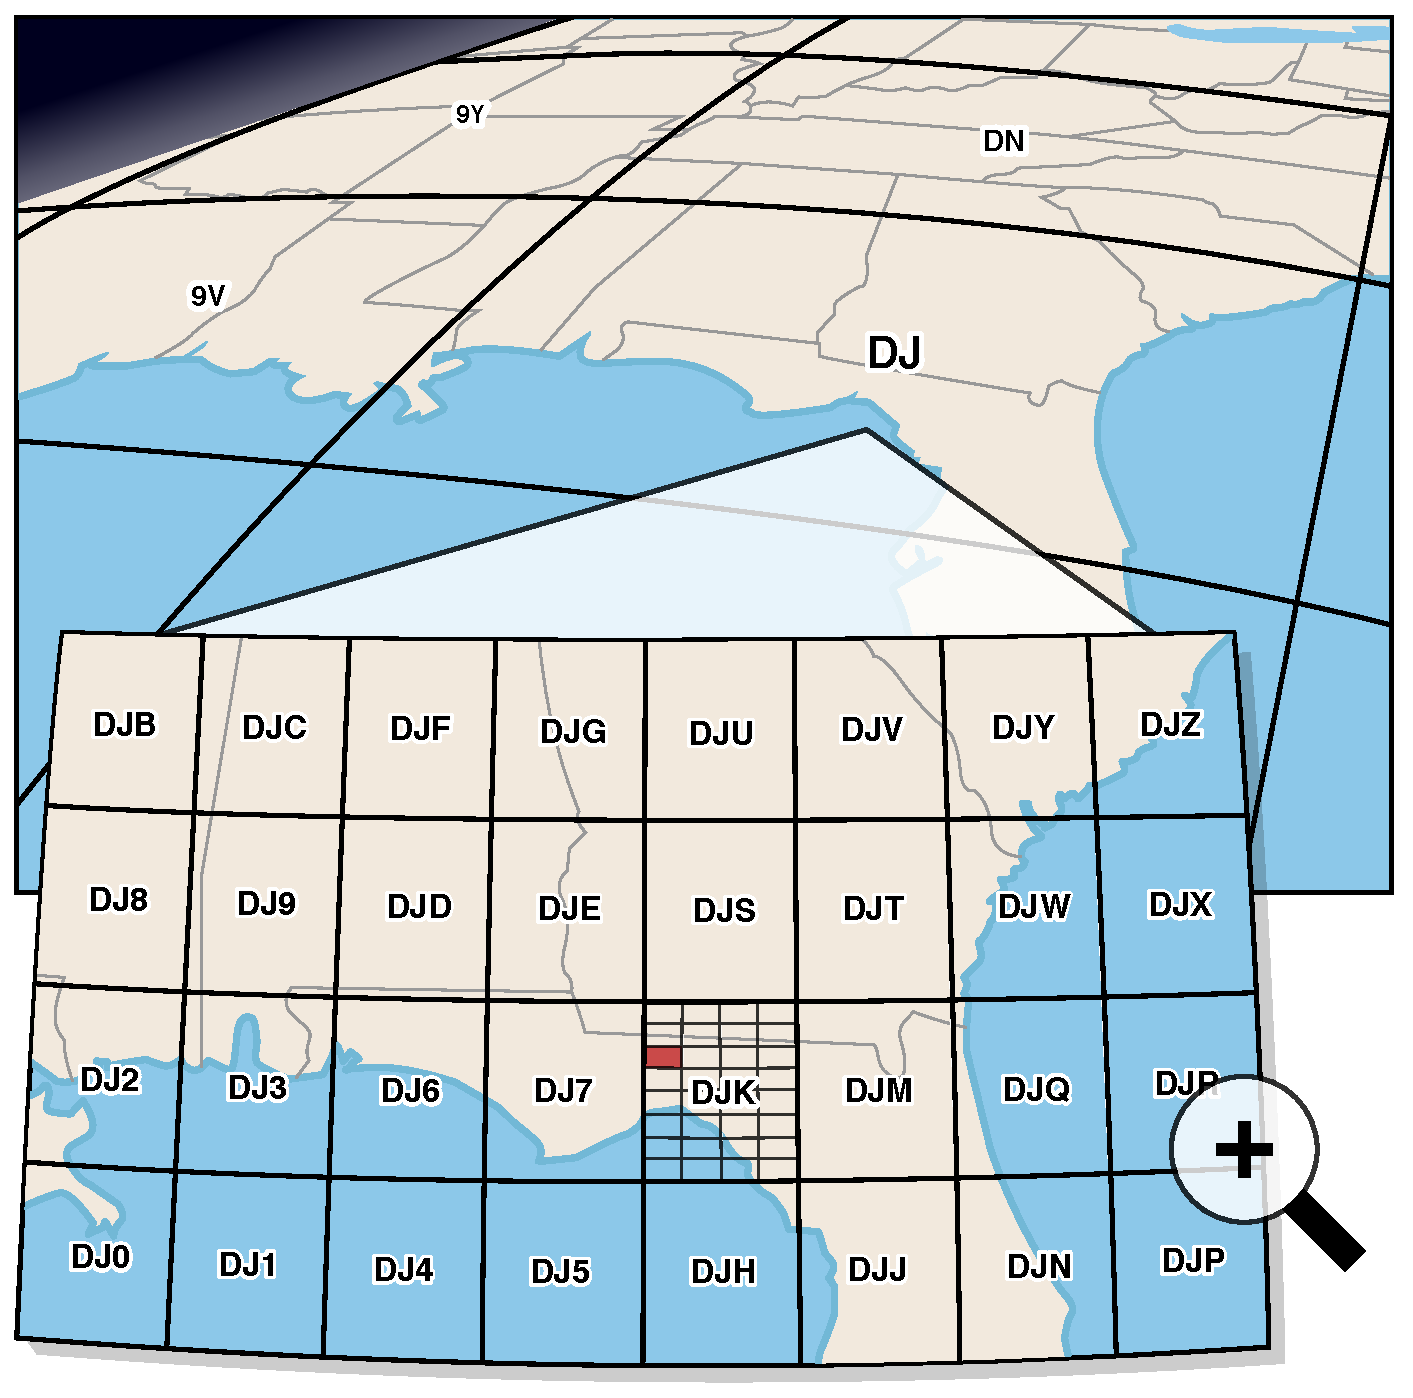
\includegraphics[width=2.5in]{figures/geohash.pdf}}
    \caption{Visual demonstration of the Geohash algorithm.}
    \label{fig:geohash}
\end{figure}




\section{Methodology}
\label{sec:methodology}

\subsection{Sketch}
\begin{figure*}
    \centerline{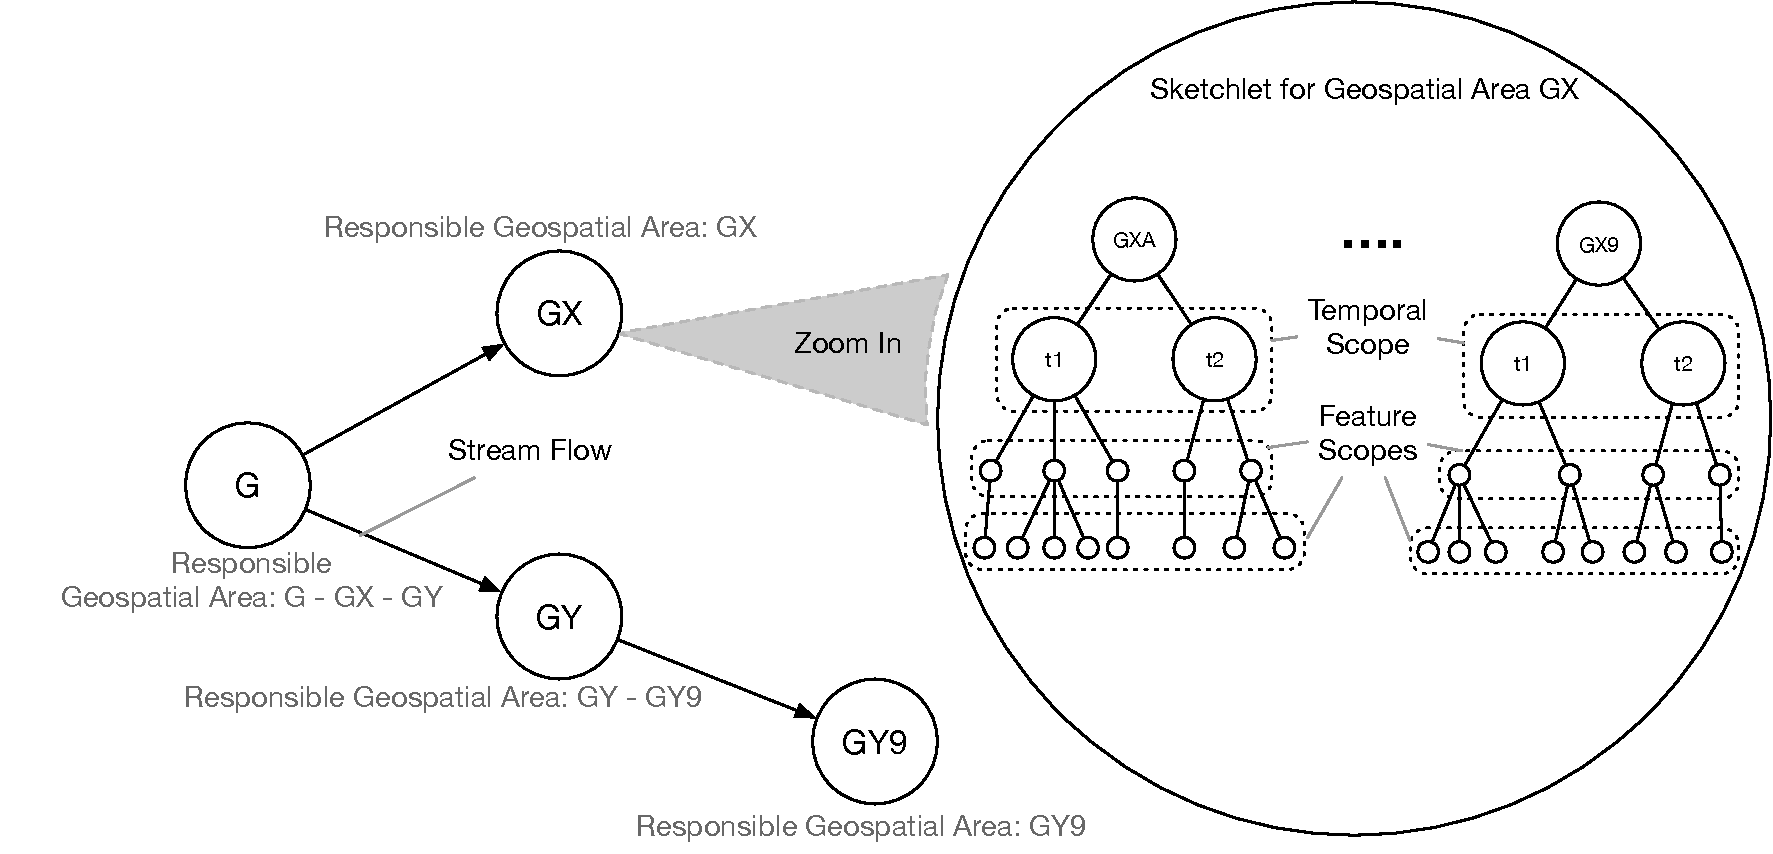
\includegraphics[width=0.8\textwidth]{figures/dist-sketch.pdf}}
    \caption{Demonstration of the distributed sketch for geospatiol region with the geohash prefix G. The sketchlets for geohash prefixes GX and GY have scaled out due to high volume of observations. A single sketchlet comprises of the SIFT data structure which is a forest of trees where each tree is responsible for a more specific geospatiol region.}
    \label{fig:dist-sketch}
\end{figure*}

The macroscopic view of the distributed sketch is one that comprises multiple sketchlets; each sketchlet executes on a different machine and is responsible for organizing data for a particular geospatial scope. The sketch is organized as a modified, distributed prefix tree. All the descendant nodes – the sketchlets – share a common prefix associated with the parent. Unlike traditional prefix trees, where the root node is an empty string, the root node is the coarsest granularity of the geohash i.e. the prefix that is common across all observations. Within a sketchlet all observations share the prefix associated with that sketchlet.

The sketch must be performant and flexible while being amenable to scaling operations. The sketch initiates scale-out operations to relieve memory pressure and preserve performance in the face of voluminous data. Scale-in operations are initiated by the sketch to conserve memory. Any sketchlet may serve as the conduit for incoming queries or analytic operations over the sketched spatiotemporal data: the sketch must be organized such that the sketchlets are not involved in redundant query evaluations or analytic operations. 

The geohash algorithm is well suited to our problem and plays a central role in the organization of the distributed sketch. Since the geohash algorithm represents a bounding box, it faciliates collation of observations from a particular geographical scope. This in turn allows us to redirect queries effectively and ensure data locality during query evaluations. Increases in the length of the geohash string correspond to geographically smaller bounding boxes being identified with increasing precision. This is also well-aligned with dynamic scaling maneuvers performed by the sketch to manage memory requirements and the availability of observational data. Scaling operations within the sketch are targeted. Scale-out operations target geospatial locations with increased density of observations to relieve memory pressure and alleviate performance bottlenecks. Scale-in operations target geolocations where there is a sparsity in available data to conserve memory.

Each sketchlet is responsible for real-time organization, summarization, and compaction of observational data from the geographical scope represented by the sketchlet’s geohash.  The sketchlet performs two operations. First, it extracts metadata from incoming observations. Metadata extracted from individual observations include: geolocations, chronological information, and features encapsulated within the observation.

Second, the sketchlet is responsible for effective summarization and compaction of measurements and accompanying spatiotemporal information extracted in the previous step. The sketchlet organizes its summarization of the observational data, as a forest of trees in a data structure called SIFT (Summarization Involving a Forest of Trees). The underlying principle within this data structure is \textbf{grouping} to exploit similarities in values reported within observations. This organization principle extends to all dimensions associated with the observations: spatial, temporal, and encapsulated features. The grouping principle allows us to preserve fidelity of the observational space while conserving memory footprints.

Each tree within the SIFT is rooted at a higher precision geohash than that associated with the sketchlet. For example, at a sketchlet with a geohash prefix, gx, the trees within the SIFT at that sketchlet are rooted at higher precision geohashes such as gxb, gxc, gxd, etc. An advantage of this approach is that the sketchlet partitions data from different regions within the larger geospatial scope into smaller regions. This partitioning allows the data structure to further exploit similarity in the observation values reported for that spatial scope. 

Within each SIFT tree, the second level is used to group observations based on their temporal properties. This approach allows us to exploit similarity in readings reported for a particular time-range. Note that as you traverse one of the trees within the forest, this organization means that all descendants of a temporal node correspond to measurements reported for a particular region for a particular temporal scope. The SIFT data structure also allows supporting finer-grained temporal resolutions for the recent past –- e.g., minutes, hours, day, weeks, etc. – and then target compaction operations that fold finer-grained temporal scopes into a coarser grained temporal scope as time advances. Specifically, our organizational structure that allows us to support varying levels of expressiveness for different temporal scopes – recent observations are represented more expressively. For example, on 3/2/2017 we may maintain subtrees at the minute level for 3:01 pm, 3:02 pm, etc., at 3/2/2017 @ 5:00 pm these subtrees will be folded into observations for the hourly temporal scope for 3:00-4:00 pm, and at 4:00 pm the next day (3/3/2017) these would then be folded into the coarser gained temporal bin for the previous day. 

The grouping concept also extends to individual features. Each feature occupies a level within an individual tree in SIFT. At each level, the range of values that a feature can take is broken up into a set of bins (corresponding to the range of values) that they take. These ranges are determined using a KDE function to ensure that the binning of features is representative of the observed density in the distribution of values for that feature at the particular spatiotemporal scope. Each node (or bin) maintains 5 variables min, max, standard deviation, mean, and the total number of observations to capture the values observed over that bin.  This is useful during the creation of synthetic datasets that are representative of the observational space for a particular spatiotemporal scope. A simplified version of the distributed sketch only for geospatial region with prefix G is depicted in Figure~\ref{fig:dist-sketch}. 

Our methodology of grouping and organizing the summarization information as a forest of trees accomplishes two key objectives. First, it captures the distribution of feature values across a spatiotemporal scope. Second, it supports targeted reductions in the observational data volumes while being representative of the observed feature values. This is in contrast to a random sampling scheme, which may be unable to recreate distributions with high fidelity for arbitrary spatiotemporal scopes or may drop significant values.

The organization of the sketchlet is such that it is amenable to scale-out and scale-in operations of the distributed sketch. Perhaps the most important feature provided by the SIFT data structure is support for scaling operations. For example, if a subregion – represented by a tree within the forest maintained at each sketchlet – has a higher density (and variability) of the reported observational values, that tree would have a correspondingly disproportionate memory footprint within the data structure. This allows us to target scaling maneuvers to particular sub-regions managed at a sketchlet to alleviate memory pressure.  During scale-in operations, descendants can be folded into the parent – the descendant’s SIFT is simply added as a tree to the SIFT maintained at the parent.

\subsection{Stream Partitioning}
We use the Geohash~algorithm~\cite{geohash} to balance load and partition incoming data streams across processing resources. Geohash divides the earth into a hierarchy of bounding boxes identified by Base 32 strings; the longer the Geohash string, the more precise the bounding box. Figure~\ref{fig:geohash} illustrates this hierarchy; most of the western United States and Mexico are contained within the bounding box described by Geohash string \emph{9}, while \emph{9Q} encompasses parts of California, Nevada, Arizona, and Utah. The bounding box \emph{9Q9K} (highlighted in red) contains San Jose, California. This hierarchical representation enables \textsc{Rivulet} to cope with both low- and high-density regions. For instance, several resources may be tasked with managing streams originating in and around the San Francisco region, while the entirety of Yosemite National Park could fall under the purview of a single node.

\begin{figure}
    \centerline{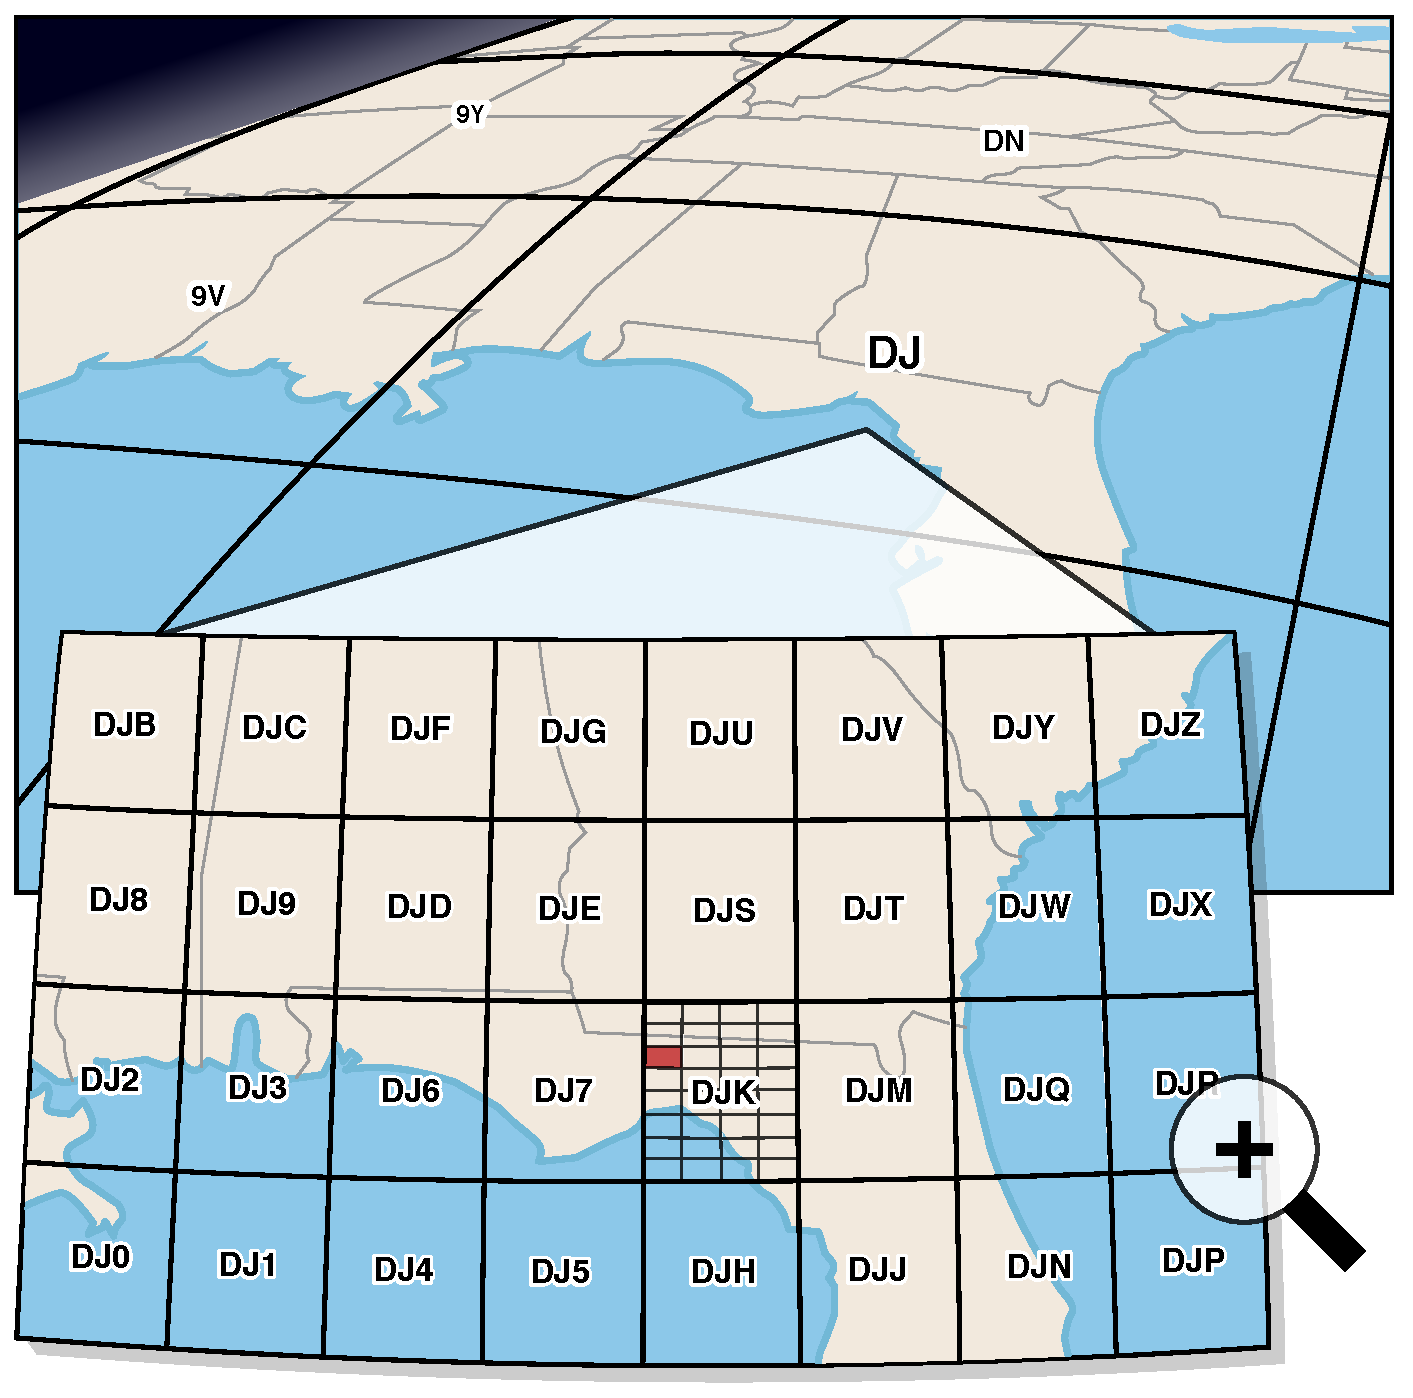
\includegraphics[width=3.5in]{figures/geohash.pdf}}
    \caption{A demonstration of the Geohash algorithm. Each additional character in a Geohash string describes a finer-grained region; Geohash \emph{9Q} contains a substantial portion of California, USA, while \emph{9Q9K} (highlighted in red) represents a smaller region containing San Jose, California.}
    \label{fig:geohash}
\end{figure}

To achieve fine-grained control over our Geohash partitions, we operate at the bit level rather than Base 32 character level when routing streams. Each bit added to a Geohash string reduces its scope by half, with each character represented by five bits ($2^5 = 32$). In other words, a four-character Geohash string represents 20 spatial subdivisions. This property allows us to manage and allocate resources across a wide variety of observational densities.

 % This needs to be moved as we get the paper structure finalized

\subsection{Coping with High Data Rates: Scaling out}
\label{subsec:scaling-out}
There are two primary approaches to scaling a node that is experiencing high traffic: \emph{replication} and \emph{load migration}. In replication-based scaling, new nodes are spawned during high data arrival rates that are responsible for identical spatial scopes as their originating node. Assimilation of the newly-created node involves partitioning inbound streams directed to the original node. The upstream node is responsible for this partitioning, which may be performed in a skewed fashion with the new node receiving a larger portion of the inbound stream.  Alternatively, inbound streams to the original node may also be partitioned in a round-robin fashion between the original and the newly-created node.

In targeted load migration, particular geospatial scopes are evicted from the original node to the newly created node during heavy traffic. Deciding which spatial scopes to migrate is based on data arrival rates and the rates at which particular portions of the sketch are being updated.

%[malensek] NOTE: I removed this because it contradicts our discussion on the ability of the sketch to merge arbitrary states (even duplicated state -- in fact, that makes things easier). I think there are plenty of other reasons why replication-based scaling is weaker anyway.
%Replication-based scaling introduces a challenge during query evaluations in that the query must be forwarded to all nodes responsible for a particular scope and the results merged; depending on the nature of these queries (for e.g., correlation analysis and inferential queries) merging of results may be difficult to accomplish without extensive state synchronizations.
%TODO: lines about how downscaling can be difficult in replication settings

In \textsc{Synopsis}, we use targeted load migration for scaling out.
Our implementation closely follows the MAPE loop~\cite{maurer2011revealing} which is comprised of four phases: monitor (M), analyze (A), planning (P) and execution (E).
%The monitoring task as shown in Figure~\ref{fig:process-monitor} periodically probes every \textsc{Synopsis} task to gather two performance metrics as part of monitoring phase.
A monitoring task periodically probes every node to gather two performance metrics:
\begin{enumerate}[leftmargin=*]
	\item Length of the backlog: This represents the number of unprocessed messages in the queue. If the \textsc{Synopsis} task cannot keep up with the incoming data rate, then the backlog will grow over time.
	\item Memory pressure: Each node is allocated a fixed amount of memory. 
	Exceeding these memory limits creates memory pressure, which may cause extended garbage collection cycles and increased paging activity. 
	This will eventually lead to reduced performance in every \textsc{Synopsis} task running on the node.
	The monitoring task records memory utilization of the process as well as its individual tasks.
\end{enumerate} 

The objective of scaling out is to maintain the \emph{stability} of each node.
We define stability as the ability to keep up with incoming data rates while incurring a manageable memory pressure.  During the analysis phase, we use threshold-based rules \cite{lorido2012auto} to provide scale out recommendations to \textsc{Synopsis} nodes.
We rely on a reactive scheme where the rules are evaluated on current observations.
Scaling out recommendations are provided if either of the following rules are consistently satisfied for a certain number of observations:
\begin{itemize}[leftmargin=*]  
\item Backlog growth, which indicates that a portion of the load needs to be migrated to a different \textsc{Synopsis} node.
\item High overall memory utilization above a threshold, which is usually set below the memory limits to allow a capacity buffer for the process to avoid oscillation.
\end{itemize}

Upon receiving a scaling out recommendation from the monitoring task, the \textsc{Synopsis} node executes the planning and execution phases.
During the planning phase, the node chooses portion(s) of the region within its current purview to be handed over to another node.
For this task, the node relies on metadata it maintains for each subregion (corresponding to longer Geohash strings) and a numeric value provided by the scale out recommendation that measures how much load should be migrated.
This metadata includes the data rate and the timestamp of the last processed message for each subregion.
A \textsc{Synopsis} node updates these metadata records with each message it processes.
Nodes often migrate several prefixes during a scale out operation.

Only a single scale out operation takes place at a given time per node, which is controlled by a mutex lock.
Further, every scaling operation is followed by a stabilization period where no scaling operation takes place and system does not enter the monitoring phase for the next MAPE cycle.
The objective of these constraints is to avoid oscillations in scaling activities; for instance, aggressively scaling out in the presence of memory pressure could result in underprovisioning, which would then lead to aggressive downscaling.

Figure~\ref{fig:scale-out-protocol} depicts the phases of the scale out protocol.
Once the \textsc{Synopsis} node decides on subregions to scale, it initiates the scale out protocol by contacting the \emph{deployer} node, which is responsible for launching tasks.
In this message, it includes a list of preferred \textsc{Synopsis} nodes for the load migration as well as memory requirements and expected message rate for the load.
The preferred node set includes the \textsc{Synopsis} nodes that already hold other subregions.
The objective here is to minimize the number of nodes responsible for each geographical region to reduce communication during query evaluations.

The \textsc{Synopsis} deployer component has an approximate view of the entire system gathered through gossip messages, which includes the memory pressure and cumulative backlog information for each node.
Based on this view and the information present in the request, the deployer replies back with a set of target \textsc{Synopsis} nodes.
If a suitable node cannot be found, a new node will be launched that includes the location in question.
Upon receiving a response from the deployer, the node that is scaling out contacts the target node and tries to acquire the mutex.
A lock will be granted if the target can accommodate the load and no other scaling operations are taking place.
If the lock acquisition fails, another node from the list is attempted; otherwise, the original \textsc{Synopsis} node will create a pass-through channel and direct traffic towards the target node.
Once this process is complete, the source node will initiate a state transfer asynchronously using a background channel to ensure the stream data flow is not affected, and update its memory utilization metrics to account for the pending state transfer.
%Completing the scale out protocol quickly is important because it can release mutual exclusive locks in both origin and target \textsc{Synopsis} nodes quickly and participate in other scaling activities soon after the stabilization period.
%
\begin{figure}
    \centerline{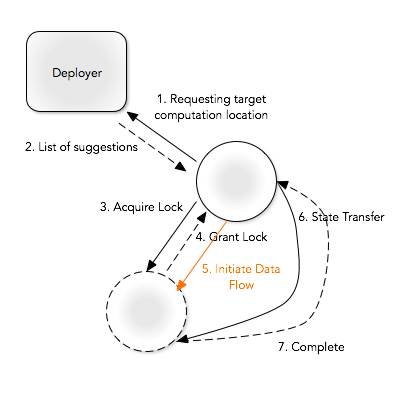
\includegraphics[scale=0.55]{figures/scale-out-protocol.png}}
    \caption{Scale out protocol}
    \label{fig:scale-out-protocol}
\end{figure}
%
\subsection{Downscaling}
\label{subsec:scaling-in}
During \emph{downscaling} (or scaling in), \textsc{Synopsis} nodes merge back some of the subregions scaled out previously.
This ensures better resource utilization in the system in addition to efficient query evaluations by having to contact fewer nodes.
Downscaling operations are also guarded by the same mutex lock used for scaling out (only one scale out or scale in operation takes place at a given time) and are followed by a stabilization period.

Monitoring and analysis during downscaling proceeds similarly to scaling out, except for the obvious change to the threshold-based rules: now both memory pressure and backlog length metrics should consistently record values below a predefined lower threshold.
When scaling in, we use a less aggressive scheme than scaling out; a single subregion is acquired during a single scale in operation.
Scaling in is more complex than scaling out because it involves more than one \textsc{Synopsis} node in most cases.
At this point, it is possible that further scale out operations have taken place in the scaled out subregion after the initial scale out.
For instance, if node A in Figure~\ref{fig:stream-partitioning} decides to scale in the subregion \emph{DJK}, then it must communicate with both nodes C and E.

The downscaling protocol starts with a lock acquisition protocol similar to scaling out as illustrated in Figure~\ref{fig:scale-in-protocol}, but locking the entire subtree is required.
As per our example, node A will have to acquire locks for nodes C and E.
Locks are acquired in a top-to-bottom fashion where parent locks itself and then attempts to lock the child.
If lock acquisition is failed in any part of the subtree, then the scale in operation is aborted and the monitoring process will start the next iteration of the MAPE loop immediately.
If the subtree is successfully locked, then data flow to the child nodes corresponding to this subregion is immediately terminated.

The state acquisition phase begins next.
To ensure that \textsc{Synopsis} does not lose any messages, the initiating node sends a \emph{termination point} control message to the child node.
The termination point is the sequence number of the last message sent to the child node either by the parent itself or by the short circuit channel.
%It may be possible that the child has already processed this message and updated its sketch by the time it receives the termination point control message, but in extreme cases the termination point control message may get processed before the actual stream packet with the same sequence number.
%This is because control plane and data plane use separate channels and also due to the possibility of data plane messages are being queued before processing.
Once the child node has processed every message up to the termination point, it sends out termination point messages to all relevant child nodes. In our example, node C sends a termination point control message to node E upon processing the stream packet corresponding to the termination point sent by node A.
After the entire subtree has seen all messages up to the termination point, they acknowledge the initiator node and start transferring their states asynchronously.
Once the parent node receives acknowledgments from the entire subtree, it starts propagating the protocol end messages to initiate lock releasing.
Locks are released from the bottom to top in the subtree, with the parent releasing its lock after each child has released its lock.

\begin{figure}
    \centerline{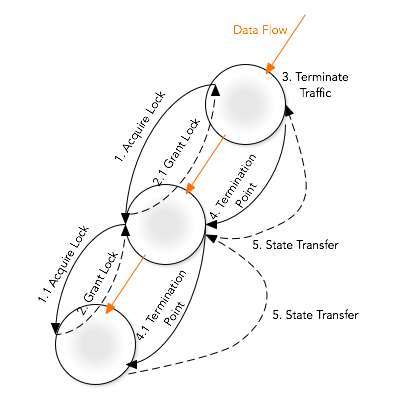
\includegraphics[scale=0.55]{figures/scale-in-protocol.png}}
    \caption{Downscaling protocol}
    \label{fig:scale-in-protocol}
\end{figure}

\subsection{Query Evaluations}
\label{subsec:query-eval}
\textsc{Synopsis} incorporates support for user-defined queries that are evaluated over the distributed sketch.  Queries can be specified by the user in a SQL-like format or with JSON-based key-value descriptions similar to GraphQL~\cite{graphql}. Exact-match, range-based, and summarization queries are all supported over spatiotemporal bounds and individual feature values. The following example depicts how SQL-like queries can be formulated for evaluation over the sketch.

\begin{Verbatim}[fontsize=\footnotesize]
SELECT MEAN(precipitation), MAX(wind_speed)
WHERE temperature > 20 AND temperature < 30
AND humidity > .8 AND CORRELATION(
    cloud_cover, precipitation) < -0.25
\end{Verbatim}

Depending on scaling operations and the spatial scope of the queries, evaluations are carried out on one or more sketchlets. Information on the placement of sketchlets in the system and their corresponding feature scopes is maintained at each sketchlet in a geohash prefix tree, with changes propagated through the network in an eventually-consistent manner as data is ingested and scaling maneuvers occur.

The entry point for these queries, called the \emph{conduit}, may be any of the sketchlets comprising the distributed sketch. During query evaluations, the first step is to identify the set of sketchlets that are relevant to the query. The conduit consults its prefix tree to locate sketchlets based on spatial, chronological, and feature constraints specified by the user. After this process is complete, the conduit forwards the queries on to the sketchlets for evaluation and supplies the client with a list of sketchlets that will respond to the query. As queries execute, results are streamed back to the client and merged by the client API. This strategy ensures that I/O and processing activities are interleaved on the client side.

Our distributed prefix tree enables query evaluations during both scaling in and out. For instance, when a conduit attempts to forward a query to a child sketchlet that is undergoing a scale-in operation, the request will be redirected to the its parent sketchlet. This process can continue recursively up through the network, ensuring queries will reach their destination.

\subsubsection{Query Types}
Queries supported by \textsc{Synopsis} fall into six categories:
\begin{description}[leftmargin=*]
    \item[Relational Queries] describe the feature space in the context of the hierarchical trees within our SIFT data structure and may target ranges of values under certain conditions. For example, ``What is the relationship between temperature and humidity during July in Alaska, USA, when precipitation was greater than 1 centimeter?'' These queries return a subset of the overall sketch that includes any other matching feature values as well.
    % Subsketches may be manipulated and inspected on the client side, and then reused in subsequent queries to request more detail or broaden the query scope. Relational queries can optionally return statistical metadata stored in the leaf nodes of the tree; this is also supported by our statistical query functionality.

    \item[Statistical Queries] allow users to explore statistical properties of the observational space. For example, users can retrieve and contrast correlations between any two features at different geographic locations at the same time. Alternatively, queries may contrast correlations between different features at different time ranges at the same geographic location. These queries also support retrieval of the mean, standard deviation, and feature outliers based on Chebyshev's inequality \cite{knuth1968art}.

    \item[Density Queries] support analysis of the distribution of values associated with a feature over a particular spatiotemporal scope. These include kernel density estimations, estimating the probability of observing a particular value for an observation, and determining the deciles and quartiles for the observed feature.% Kernel density estimations can request the function itself, an integral over a range of values, or the probability of a single value.

    \item[Set Queries] target identification of whether a particular combination of feature values was observed, estimating the cardinality of the dataset, and identifying the frequencies of the observations. Each type of set query requires a particular data structure, with instances created across configurable time bounds (for instance, every day). Set membership is determined using space-efficient bloom~filters~\cite{bloom1970space}, while cardinality (number of distinct elements) queries are supported by the HyperLogLog~\cite{flajolet2007hyperloglog} algorithm.

%To determine set membership, we use Bloom filters may produce false positives, but never false negatives. Besides returning a \texttt{true} or \texttt{false} result to the user, membership queries also include the probability of the answer being a false positive.  Set HyperLogLog is able to estimate cardinality with high accuracy and low memory consumption. Finally, observation frequencies are provided by the count-min data structure \cite{cormode2005improved}. Count-min is structurally similar to a bloom filter, but can be used to estimate the frequency of values within a particular error band. Frequency queries are accompanied by their associated confidence intervals and relative error.

\item[Inferential Queries] enable spatiotemporal forecasts to be produced for a particular feature (or set of features). Discrete inferential queries leverage existing information in the distributed sketch to make predictions; aggregate metadata stored in the leaves of the tree can produce two-dimensional regression models that forecast new outcomes across each feature type when an independent variable of interest changes.

%In their continuous form, inferential queries are backed by machine learning models that are \emph{installed} for a particular time window and can be trained using either the sketch or new, full-resolution values as they arrive. Continuous inferential queries can stream predictions back to the client on a regular interval, or a subsequent query can reference a particular model and parameterize it to make a single prediction. Our current implementation of \textsc{Synopsis} supports multiple linear regression, but our machine learning interface allows new models to be plugged into the system at run time.

\item[Synthetic Data Queries] allow users to request the system to generate representative datasets based on the distributions stored in the sketch. Synthetic data is generated in an online fashion by sampling from the underlying distributions and then streamed to client applications for analytics. The size of the dataset may also be specified; for instance, 10\% of the volume of the original data points.
\end{description}
%
\begin{table}[h!]
    \renewcommand{\arraystretch}{1.2}
    \caption{Local sketchlet evaluation times for each query type (averaged over 1000 iterations). \vspace{-1em}}
    \label{tbl:query-times}
    \begin{center}
        \begin{tabular}{|l|c|c|}
            \hline
            \textbf{Query Type}      & \textbf{Mean (ms)} & \textbf{Std. Dev. (ms)} \\
            \hline
            Density                  & 0.007                    & 0.005 \\
            \hline
            Set Cardinality          & 0.154                    & 0.088 \\
            \hline
            Set Frequency            & 0.036                    & 0.019 \\
            \hline
            Set Membership           & 0.015                    & 0.009 \\
            \hline
            Statistical               & 0.002                    & 0.001 \\
            \hline
            \hline
            Tree Only (5 km)        & 46.357                   & 1.287 \\
            \hline
            Tree + Meta (5 km)      & 40.510                   & 6.937 \\
            \hline
            Tree + Meta (25 km)     & 47.619                   & 6.355 \\
            \hline
            Tree + Meta (800 km)    & 53.620                   & 6.818 \\
            \hline
        \end{tabular}
    \end{center}
\end{table}
Table~\ref{tbl:query-times} outlines local tree traversal times for query evaluations. These queries were separated into two groups: conventional lookups and tree retrievals. Conventional lookups include density queries, set queries, and statistical queries, while tree retrievals request targeted portions of the overall feature space as a tree.  Note that while conventional lookups do not return a tree structure to the client, they still require a tree traversal to resolve. In general, tree retrievals consume more processing time due to their serialization and I/O costs; however, it is worth noting that varying the geographical scope across sketchlet sizes from 5km to 800km did not result in a proportionate increase in processing time. Overall, the sketch provides low-latency query evaluations for each query type.


\subsection{Coping with Failures in Synopsis}
\textsc{Synopsis} relies on passive replication to recover from sketchlet failures because active replication increases resource consumption significantly and it is infeasible to use upstream backups because the state of a sketchlet depends on the entire set of messages it has processed previously \cite{castro2013integrating}.

Support for fault tolerance is implemented by augmenting the distributed sketch with a set of secondary sketchlets.
A sketchlet is assigned a set of $n$ secondary sketchlets on different machines to ensure \textsc{Synopsis} can withstand up to $n$ concurrent machine failures.
In our implementation, we used two secondary sketchlets ($n=2$) assigned to each sketchlet.
A primary sketchlet periodically sends the changes to its in-memory state as an \emph{edit stream} to its secondary sketchlets.
The secondary sketchlets, which act as the sink to the edit stream, serialize incoming messages to persistent storage.
This incremental checkpointing scheme consumes less bandwidth compared to a periodic checkpointing scheme that replicates the entire state \cite{castro2013integrating}.
By default, \textsc{Synopsis} uses the disk of the machine executing the secondary sketchlet as the persistent storage, but highly-available storage implementations such as HDFS~\cite{borthakur2008hdfs} can be used if necessary.
To reduce resource footprints, secondary sketchlets do not load the serialized state into memory unless they are promoted to being a primary.

System-wide incremental checkpoints are orchestrated by a special control message emitted by the stream ingesters.
\textsc{Synopsis} uses upstream backups at stream ingesters to keep a copy of the messages that entered the system since the last successful checkpoint.
In case of a failure, all messages since the last checkpoint will be replayed.
Sketchlets are implemented as idempotent data structures using message sequence numbers, hence they will process a replayed message only if it was not processed before.
The interval between incremental checkpoints can be configured based on time or the number of emitted messages.
Frequent checkpoints can incur high overhead, whereas longer periods between successive checkpoints consume more resources for upstream backups and require longer replay durations in case of a failure.

Membership management is implemented using Zookeeper~\cite{hunt2010zookeeper}, which is leveraged to detect failed sketchlets.
Upon receiving notification of a primary sketchlet failure, a secondary sketchlet assumes the role of primary through a leader election algorithm.
The secondary will start processing messages immediately and begins populating its state from persistent storage in the background.
Given this mode of operation, there may be a small window of time during which the correctness of queries are impacted.
This is rectified once the stored state is loaded to memory and the replay of the upstream backup is completed.
The SIFT's support for merge operations as well as its ability to correctly process out of order messages is useful during the failure recovery process.

As per our fault tolerance scheme, the \textit{total time to recover from the failure} ($T_{total}$) can be modeled as follows.
\begin{align*}
    T_{total} &= T_{d} + \max{(T_{l}, T_{r})}      
\end{align*}
where $T_{d}$ = \textit{time to detect a failure}, $T_{l}$ = \textit{time to load persisted state} and $T_{r}$ = \textit{replay time for messages at the upstream node}.

The time required to detect failures mainly depends on the session timeout value used by Zookeeper to detect lost members and the delay in propagating the notification to other members. With a $5s$ session timeout in an active cluster, we observed a mean notification propagation delay of $5.5s$ (std. dev. = $0.911s$, $95^{th}$ percentile = $6.000s$). Configuring a lower session timeout will increase the chance of false positives if sketchlets become non responsive for a while due to increased load or system activities such as garbage collection. The time required to load the persisted storage depends on the size of the serialized sketchlet; we benchmarked the time it takes to repopulate the state in all sketchlets after ingesting NOAA data for 2014. The mean state re-population time was recorded as $16.602s$ with std. dev. = $23.215s$ and $95^{th}$ \%ile = $70.877s$. Replay time mainly depends on the checkpointing interval as well as the message ingestion rate. With a checkpointing interval of 10000 messages, we experienced a mean value of $0.662s$ (std. dev. = $0.026s$, $95^{th}$ \%ile = $0.707s$) to replay an upstream buffer.



\section{Performance Evaluation}
\label{sec:performance}
To evaluate \textsc{Synopsis}, we used a real-world dataset to populate the distributed sketch. This includes dynamic scaling and an analysis of node stability as scaling operations take place, as well as query evaluation latencies for each query type.

\subsection{Dataset and Experimental Setup}
Our subject dataset was sourced from the NOAA North American Mesoscale (NAM) Forecast System \cite{noaa_nam}.  The NAM collects atmospheric data several times per day and includes features of interest such as surface temperature, visibility, relative humidity, snow, and precipitation. Each observation in the dataset also incorporates a relevant geographical location and time of creation. This information is used during the data ingest process to partition streams across available computing resources and preserve temporal ordering of events.

Our performance evaluation was carried out on a 75-node heterogeneous cluster consisting of 45 HP DL160 servers (Xeon E5620, 12 GB RAM) and 30 HP DL320e servers (Xeon E3-1220 V2, 8 GB RAM) running Fedora 23. \textsc{Synopsis} was executed under the OpenJDK Java runtime, version 1.8.0\_72.

\subsection{Dynamic Scaling}
\begin{figure}
    \centerline{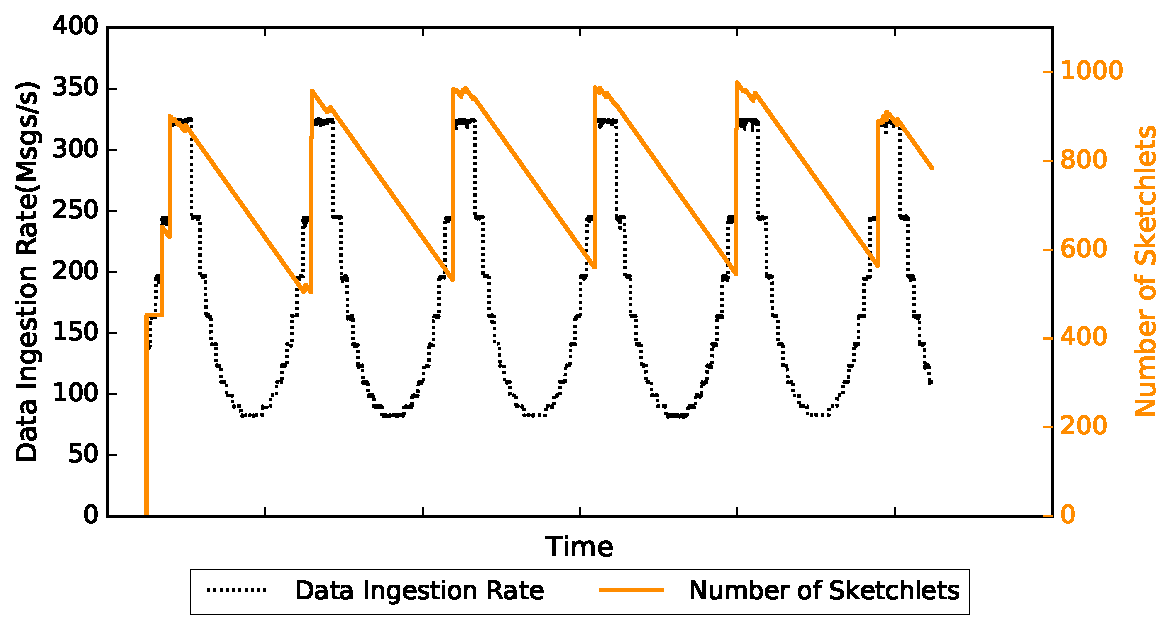
\includegraphics[width=3.5in]{figures/dyn-scaling.pdf}}
    \caption{The variation of number of sketchlets with the data ingestion rate.}
    \label{fig:dyn-scaling}
\end{figure}
We evaluated how \textsc{Synopsis} dynamically scales when the data ingestion rate is varied.
The data ingestion rate was varied over time such that the peak data ingestion rate is less than the highest possible throughput that will create a backlog at \textsc{Synopsis} nodes.
We used the number of sketchlets created in the system to quantify the scaling activities.
If the system scales out, more sketchlets will be created in child nodes after the targeted load migration.
We started with a single \textsc{Synopsis} node and allowed the system to dynamically scale.
As can be observed in Figure~\ref{fig:dyn-scaling}, the number of sketchlets varies with the ingestion rate.
Since we allow aggressive scale out, it shows a rapid scale out activity during high data ingestion rates whereas scaling in takes place gradually with one sub region (hence one sketch) at a time.
% scale out graph
\begin{figure*}[h!]
    \centerline{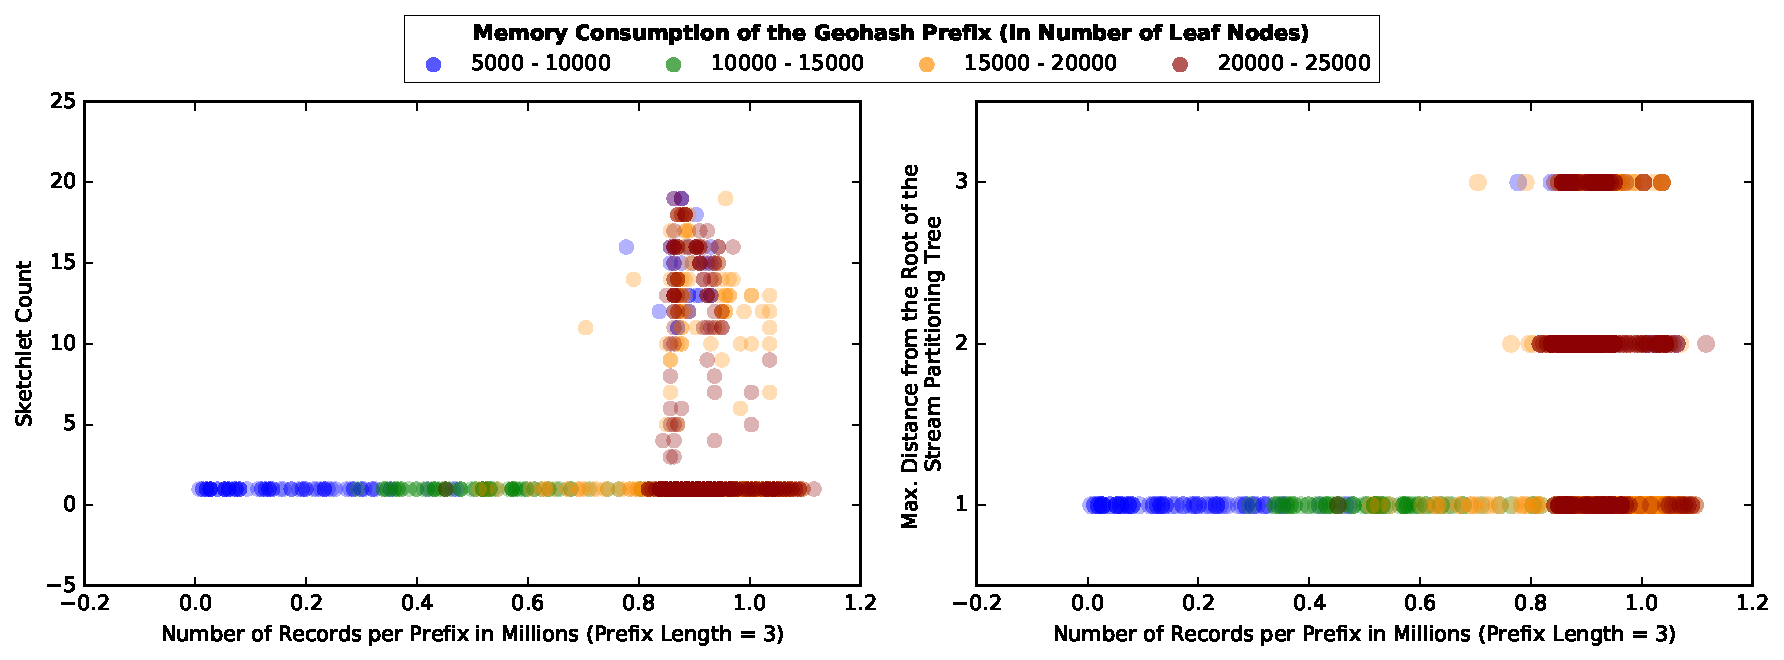
\includegraphics[width=\linewidth]{figures/scaleout_graph_analysis.pdf}}
    \caption{Analysis of a snapshot of the stream processing graph during data ingestion demonstrating the size and distribution of the information corresponding to different prefixes against the observed record count. If the information is dispersed over multiple sketchlets, it is likely to be a prefix with higher number of records and/or a wide range of observed values.}
    \label{fig:scaleout-graph-analysis}
\end{figure*}

Figure~\ref{fig:scaleout-graph-analysis} visualizes a snapshot of the stream processing graph in runtime which validates our dynamic scaling implementation. 
This represents the state of the system after consuming the complete NOAA dataset for 2014 and the graph contained 48 sketchlets. 
It shows the distribution and size of the information maintained across \textsc{Synopsis} nodes for each geohash prefix of length 3 against the number of records processed for that particular prefix.
The memory requirement for a particular geohash prefix depends on the number of records as well as the range of the observed values for different features.
The space requirement is measured in terms of the number of leaf nodes in the corresponding sketchlets.
For the majority of the prefixes, the space requirement increases with the number of records processed for a particular prefix.
If the data for a particular prefix is distributed across multiple sketchlets, then it is more likely to be a prefix with a high number of records as shown in the first subplot.
In such cases, some of these sketchlets are created in multiple iterations of scaling out operations from their original nodes which results in a higher distance from the root in the prefix tree. This is depicted in the second sub figure of Figure~\ref{fig:scaleout-graph-analysis}.
A few prefixes with high number of records can be observed with a low memory consumption and are distributed across multiple sketchlets.
Their observations spans across a smaller range, hence requires less memory but they were chosen for scaling out operations due to their high message rates. 


\subsection{Stability at Individual Nodes}
The objective of this benchmark was to demonstrate how scaling out operations manage to maintain stability at each node under varying workload conditions.
The same setup as in previous micro benchmark was used, but the evaluation metrics captured are corresponding to an individual node instead of the entire system.
For this experiment, we have enabled only a single threshold-based rule (either backlog growth based or memory usage based) at a time to demonstrate its effectiveness.

We captured how backlog length and throughput at an individual node vary with the input rate when dynamic scaling is enabled.
The \textsc{Synopsis} node that was considered for the experiment immediately received data from stream ingesters, hence the input rate observed at the node closely resembled the varying data ingestion rate.
As shown in Figure~\ref{fig:stability-backlog}, scaling out helps a node to keep up with the variations in the workload which in turn causes the backlog to stay within a safe range.
It also demonstrates the infrequent rapid scaling out activities and the continuous gradual downscaling activities as explained in section~\ref{subsec:scaling-out}.

Figure~\ref{fig:stability-mem} demonstrates how memory consumption based threshold-based rules trigger scaling manures to maintain the system stability.
We have used a 0.45 of the total available memory for a JVM process as the upper threshold for triggering a scale out operation.
In certain occasions, it is required to perform multiple consecutive scaling out operations (interleaved with the cooling down periods) to bring the memory usage to the desired level due to the increased memory utilization caused by the data ingestion happening in the background.
% system stability
\begin{figure*}[h!]
    \begin{subfigure}{0.48\textwidth}
            \centering
            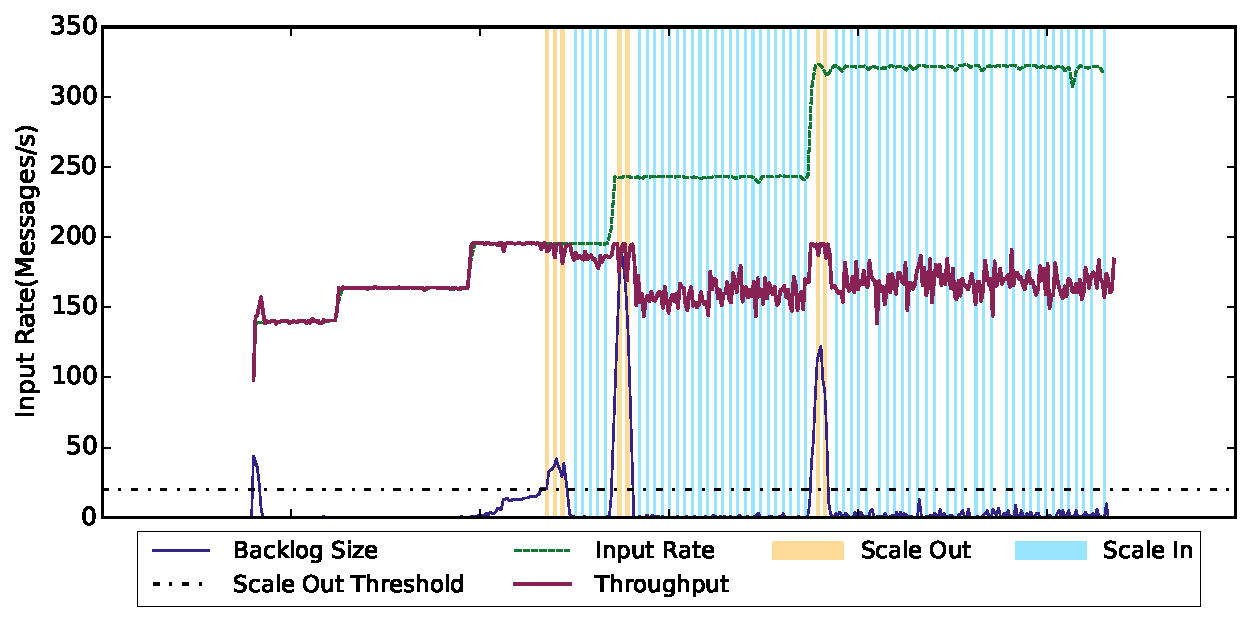
\includegraphics[scale=0.42]{figures/stability_partial.pdf}
            \caption{Dynamic scaling manures triggered by backlog growth based threshold rules}
            \label{fig:stability-backlog}
    \end{subfigure}
    \begin{subfigure}{0.48\textwidth}
            \centering
            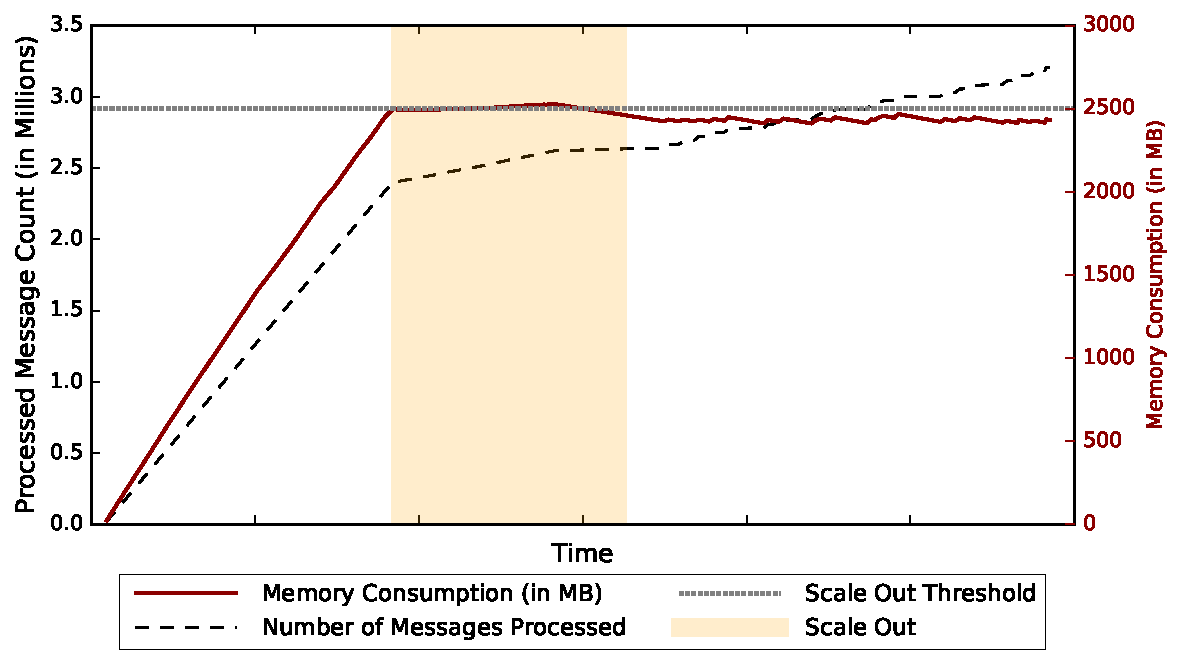
\includegraphics[scale=0.42]{figures//mem_stability.pdf} 
            \caption{Dynamic scaling manures triggered by memory usage based threshold rules}
            \label{fig:stability-mem}
    \end{subfigure}
    \caption{Scaling out enables maintaining stability at an individual node based on backlog growth and memory usage}
    \label{fig:system-stability}
\end{figure*}

\subsection{Growth of the Distributed Sketch over Time}
% system benchmark on mem. consumption
\begin{figure}[h]
    \centerline{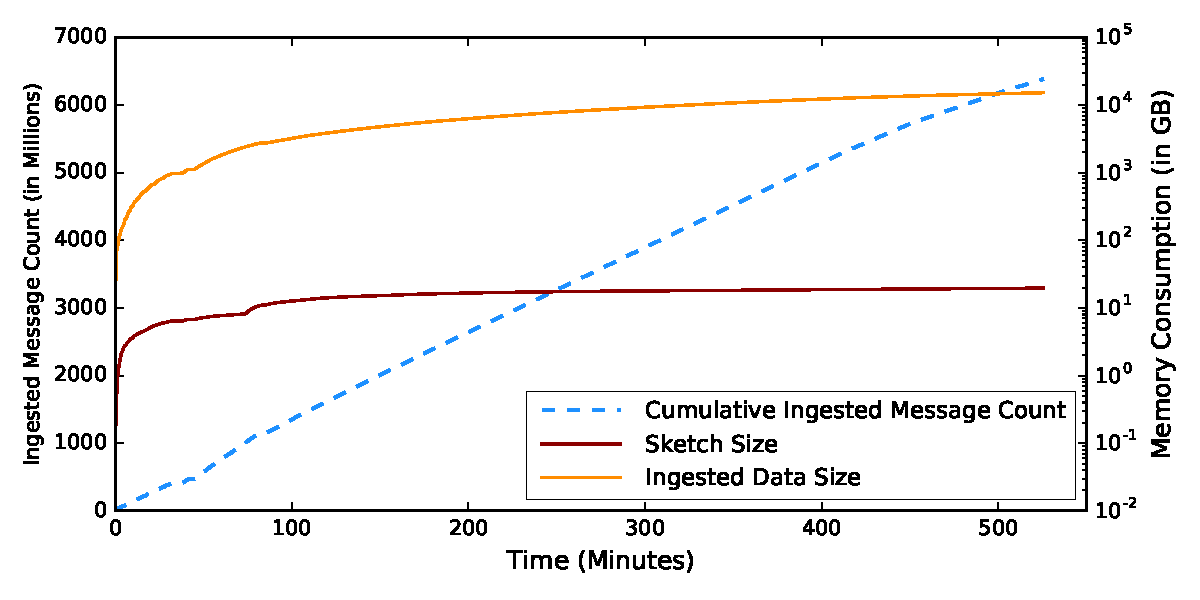
\includegraphics[width=\linewidth]{figures/ing-and-mem-usage.pdf}}
    \caption{Memory usage of the distributed sketch over time against the amount of ingested data. The rate of growth of the distributed sketch decreases over time resulting in a sketch which is multiple degrees of magnitudes smaller than the amount of ingested data}
    \label{fig:dist-sketch-mem-usage}
\end{figure}
We evaluated the growth in memory consumption of the distributed sketch over time with continous data ingestion as shown in Figure~\ref{fig:dist-sketch-mem-usage}.
The rate of growth of the distributed sketch is decreased overtime.
At the end of our monitoring period, the ingested data size was over three magnitudes higher ($\sim 1285$) than the sketch size. 


\subsection{Sketch Query Evaluation}
To evaluate the performance of the sketch, we executed several representative query workloads across a variety of sketchlet sizes. These queries were separated into two groups: data structure lookups and graph lookups. Data structure lookups include density queries, set queries, and summary statistics for the entire sketch, while graph lookups involve targeted portions of the overall feature space. In general, queries that require a graph lookup consume more processing time, but are much more expressive; for instance, such a query could request summary statistics or feature relationships when the temperature is between 20 to 30 degrees, humidity is above 80\%, and the wind is blowing at 16 km/h, while a data structure lookup would be restricted to chronological parameters and select features of interest. Table~\ref{tbl:query-times} outlines the query times for both evaluation types. In general, data structure lookup operations require minimal processing. While graph lookups take longer to complete, it is worth noting that varying the geographical scope across sketchlet sizes from 5km to 800km did not result in a proportionate increase in processing time. Overall, the sketch is able to satisfy our goal of low-latency query evaluations for each query type.

\begin{table}[h!]
    \renewcommand{\arraystretch}{1.4}
    \caption{Query evaluation times for each query type (averaged over 1000 iterations).}
    \label{tbl:query-times}
    \begin{center}
        \begin{tabular}{|l|c|c|}
            \hline
            \textbf{Query Type}      & \textbf{Eval. (ms)} & \textbf{Std. Dev.} \\
            \hline
            Density                  & 0.007                    & 0.005 \\
            \hline
            Set Cardinality          & 0.154                    & 0.088 \\
            \hline
            Set Frequency            & 0.036                    & 0.019 \\
            \hline
            Set Membership           & 0.015                    & 0.009 \\
            \hline
            Statistics               & 0.002                    & 0.001 \\
            \hline
            \hline
            Subgraph Stat. (5 km)    & 46.357                   & 1.287 \\
            \hline
            Relational (5 km)        & 40.510                   & 6.937 \\
            \hline
            Relational (25 km)       & 47.619                   & 6.355 \\
            \hline
            Relational (800 km)      & 53.620                   & 6.818 \\
            \hline
        \end{tabular}
    \end{center}
\end{table}
% distributed query evaluation
\begin{figure*}
    \centerline{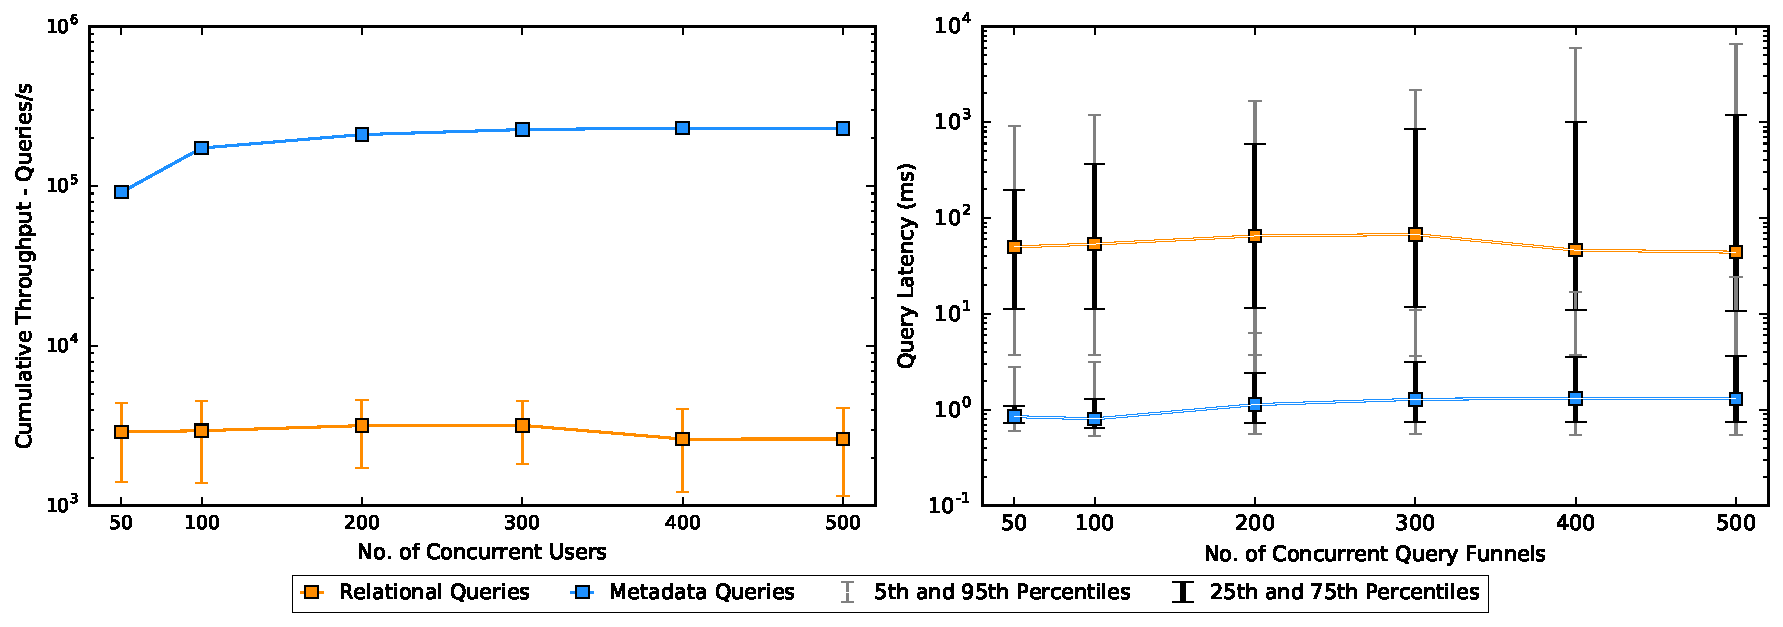
\includegraphics[width=\linewidth]{figures/query_benchmark_both.pdf}}
    \caption{Distributed Query Evaluation Performance. Variation of cumulative throughput and latency against the number of concurrent query funnels in a 40 node \textsc{Synopsis} cluster.}
    \label{fig:dist-query}
\end{figure*}

Figure~\ref{fig:dist-query} demonstrates the efficiency of the query evaluations over the distributed sketch.
Cumulative query throughput and latencies were measured with different number of concurrent query funnels.
A query funnel continously generates and dispatches random queries at their maximum possible rate.
Our setup included 40 Synopsis nodes and one of those nodes was randomly chosen as the conduit for each query.

\section{Related Work}
\label{sec:related}
Data~Cubes~\cite{gray1996data,harinarayan1996implementing,mumick1997maintenance,ho1997range} are a data structure for Online Analytical Processing that provide multidimensional query and summarization functionality. These structures generalize several operators provided by relational databases by projecting two-dimensional relational tables to N-dimensional cubes (also known as \emph{hypercubes} when $N > 3$). Variable precision in Data Cubes is managed by the \emph{drill down/drill up} operators to increase and decrease resolution, respectively, and \emph{slices} or entire cubes can be summarized through the \emph{roll up} operator. While Data Cubes provide many of the same features supported by our distributed sketch, they are primarily intended for single-host offline or batch processing systems due to their compute- and data-intensive updates. In fact, many production deployments separate transaction processing and analytical processing systems, with updates pushed to the Data Cubes on a periodic basis. 

CHAOS~\cite{gupta2009chaos} builds on Data Cubes in a single-host streaming environment by pushing updates to its \emph{Computational Cubes} more frequently. To make dimensionality and storage requirements manageable, Computational Cubes only index summaries of incoming data that are generated during a preprocessing step. However, full-resolution data is still made available through continuous queries that act on variable-length sliding windows. CHAOS builds its summaries using a wavelet-based approach, which tend to be highly problem-specific. Additionally, updates to the cube structure are still generated and published on a periodic basis rather than immediately as data is assimilated.

Galileo~\cite{malensek2016analytic,malensek2015fast} is a distributed hash table that supports the storage and retrieval of multidimensional data. Given the overlap in problem domain, Galileo is faced with several of the same challenges as \textsc{Synopsis}. However, the avenues for overcoming these issues diverge significantly due to differences in storage philosophy: \textsc{Synopsis} maintains its dataset completely in main memory, avoiding the orders-of-magnitude disparity in I/O throughput associated with secondary storage systems. This makes \textsc{Synopsis} highly agile, allowing on-demand scaling to rapidly respond to changes in incoming load. Additionally, this constraint influenced the trade-off space involved when designing our algorithms, making careful and efficient memory management a priority while striving for high accuracy.

Simba (Spatial In-Memory Big data Analytics)~\cite{xiesimba} extends Spark SQL~\cite{armbrust2015spark} to support spatial operations in SQL as well as DataFrames. It relies on data being stored in Spark~\cite{zaharia2010spark}. Even though this approach provides a high accuracy, it is not scalable for geospatial streams in the long term due to high storage requirements. In \textsc{Synopsis}, spatial queries can be executed with a reasonable accuracy without having to store the streaming data as-is.

Dynamic scaling and elasticity in stream processing systems has been studied thoroughly \cite{heinze2014auto, gulisano2012streamcloud, castro2013integrating, loesing2012stormy, heinze2013elastic, schneider2009elastic}.
Heinze et al.~\cite{heinze2014auto} explores using different dynamic scaling schemes including threshold-based rules and reinforcement learning using the FUGU~\cite{heinze2013elastic} stream processing engine.
Based on these schemes, the operators are continuously migrated between hosts in a FUGU cluster in order to optimize the resource utilization and to maintain low latency.
Their approach is quite different from ours, because in \textsc{Synopsis} we perform a targeted load migration where the workload of a computation is dynamically adjusted instead of entirely moving it to a host with a higher or lower capacity than the current host.
Further, we do not interrupt the data flow through \textsc{Synopsis} when dynamic scaling activities are in progress, whereas in FUGU the predecessor operator is temporarily paused until operator migration is complete. 

StreamCloud~\cite{gulisano2012streamcloud} relies on a global threshold-based scheme to implement elasticity where a query is partitioned into sub-queries which run on separate clusters.
StreamCloud relies on a centralized component, the Elastic Manager, to initiate the elastic reconfiguration protocol, whereas in Synopsis each node independently initiates the dynamic scaling protocol.
This difference is mainly due to different optimization objectives of the two systems; StreamCloud tries to optimize the average CPU usage per cluster while \textsc{Synopsis} attempts to maintain stability at each node.
The state recreation protocol of StreamCloud is conceptually similar to our state transfer protocol, except in StreamCloud the tuples are buffered at the new location until the state transfer is complete, whereas in \textsc{Synopsis} the new node starts building the state (sketch) which is later merged with the asynchronously transferred state from the previous node.

Gedik et al.~\cite{schneider2009elastic} also uses a threshold-based local scheme similar to \textsc{Synopsis}. Additionally, this approach keeps track of the past performance achieved at different operating conditions in order to avoid oscillations in scaling activities.
The use of consistent hashing at the splitters (similar to stream partitioners in \textsc{Synopsis}) achieves both load balancing and monotonicity (elastic scaling does not move states between nodes that are present before and after the scaling activity).
Similarly, our Geohash-based partitioner together with control algorithms in \textsc{Synopsis} balance the workload by alleviating hotspots and nodes with lower resource utilization.
Our state migration scheme doesn't require migrating states between nodes that do not participate in the scaling activity, unlike with a reconfiguration of a regular hash-based partitioner.
Unlike in \textsc{Synopsis}, in their implementation, the stream data flow is paused until state migration is complete using vertical and horizontal barriers.
Finally, \textsc{Synopsis}' scaling schemes are placement-aware, meaning certain nodes are preferred when performing scaling with the objective of reducing the span of the distributed sketch.


\section{Conclusions and Future Work}
\label{sec:conclusions}
\textsc{Synopsis}, our framework for constructing a distributed sketch over spatiotemporal streams, is able to (1) maintain a compact representation of the observational space, (2) support dynamic scaling to preserve responsiveness and avoid overprovisioning, and (3) explore the observational space with a rich set of queries. Our methodology for achieving this is broadly applicable to other stream processing systems and our empirical benchmarks demonstrate the suitability of our approach.

We achieve compactness in our sketchlet instances by dynamically managing the number of vertices in the SIFT hierarchy as well as the range each vertex is responsible for. We also maintain summary statistics and metadata within these vertices to track the distribution/dispersion of feature values and their frequencies. As a result, \textsc{Synopsis} is able to represent datasets using substantially less memory (\textbf{RQ-1}). Given variability in the rates and volumes of data arrivals from different geolocations, our scaling mechanism avoids overprovisioning and alleviates situations where sketch updates cannot keep pace with data arrival rates. Memory pressure is also taken into account during replica creation as well as when scaling in and out (\textbf{RQ-2}). During evaluations, only the sketchlets that hold portions of the observational space implicitly or explicitly targeted by the query are involved, ensuring high throughput. We support several high-level query operations allowing users to locate and manipulate data efficiently (\textbf{RQ-3}).

Our future work will target support for \textsc{Synopsis} to be used as input for long-running computations. Such jobs would execute periodically on a varying number of machines and could target the entire observational space or only the most recently-assimilated records. We also plan to implement continuous queries that can autonomously evolve with the feature space.

\section*{Acknowledgments}
This research has been supported by funding (HSHQDC-13-C-B0018 and D15PC00279) from the US Department of Homeland Security, the US National Science Foundation's Computer Systems Research Program (CNS-1253908), and the Environmental Defense Fund (0164-000000-10410-100). \\


% ensure same length columns on last page (might need two sub-sequent latex runs)
% \balance

\bibliographystyle{abbrv}
\bibliography{references}

\end{document}
